%% This is an example first chapter.  You should put chapter/appendix that you
%% write into a separate file, and add a line \include{yourfilename} to
%% main.tex, where `yourfilename.tex' is the name of the chapter/appendix file.
%% You can process specific files by typing their names in at the 
%% \files=
%% prompt when you run the file main.tex through LaTeX.
\chapter{Teoretický rozbor}
Před vlastním návrhem a realizací je nezbytně nutné být seznámen alespoň se základní teorií použitých technologií a postupů. Bez této znalosti by se jednalo pouze o útržky textu a nebylo by možno zacházet do řešení komplexnější problematiky a kladení možných dalších témat pro následující výzkum a posun technologie.

\section{3D tisk a materiály}
3D tisk je na rozdíl od jiných technologií aditivní proces. Jedná se tedy o postupné přidávání základního materiálu v diskrétních krocích (vrstvách).
Technologií existuje několik a s postupným rozšiřováním možností aplikace jich stále přibývá. Pro řešení této práce byla vybrána technologie FDM vzhledem k jejímu masovému rozšíření, dostupnosti a nízkých nákladů. 

\subsection{Princip technologie FDM}
Fused deposition modeling, zkráceně FDM, případně FFF (Fused Filament Fabrication) je technologie 3D tisku využívající možnost opakovatelného přechodu mezi skupenstvími působením energie ve formě tepla termoplastických polymerních materiálů. Základní materiál ve formě filamentu (drátu) definovaného průměru, zpravidla 1.75\,mm, nebo 2.85\,mm, je vtlačován do předehřáte trysky silou $F$. Pokud teplota horké zóny trysky převyšuje teplotu skelného přechodu vtlačovaného materiálu dojde k dramatickému oslabení mezimolekulárních sil a vzniku viskózní kapaliny. Jelikož je průměr trysky velmi blízký průměru vtlačovaného filamentu, s vyjímkou jejího hrdla které je násobně menší, zpravidla 0.4\,mm, jediná možnost jak uvolnit vnitřní tlak je vytlačení kapaliny hrdlem. Jakmile teplota vytlačené kapaliny klesne pod teplotu skelného přechodu dojde k obnovení mezimolekulárních sil a materiál je opět pevnou látkou. Tento jev je obecně znám pod názvem extruze, zařízení .
Toto nám však nestačí pro vytvoření trojrozměrného objektu dle zadání. Je tedy třeba extrudér osadit na zařízení zajišťující pohyb v trojrozměrném prostoru.
Proces tisku pak probíhá pohybem extrudéru po předem definovaných trasách, zpravidla vždy v jedné vrstvě, a vytlačováním materiálu dle potřeby. Celý proces se poté opakuje dokud není dokončen zadaný objekt.
\begin{figure}[h]
\begin{center}
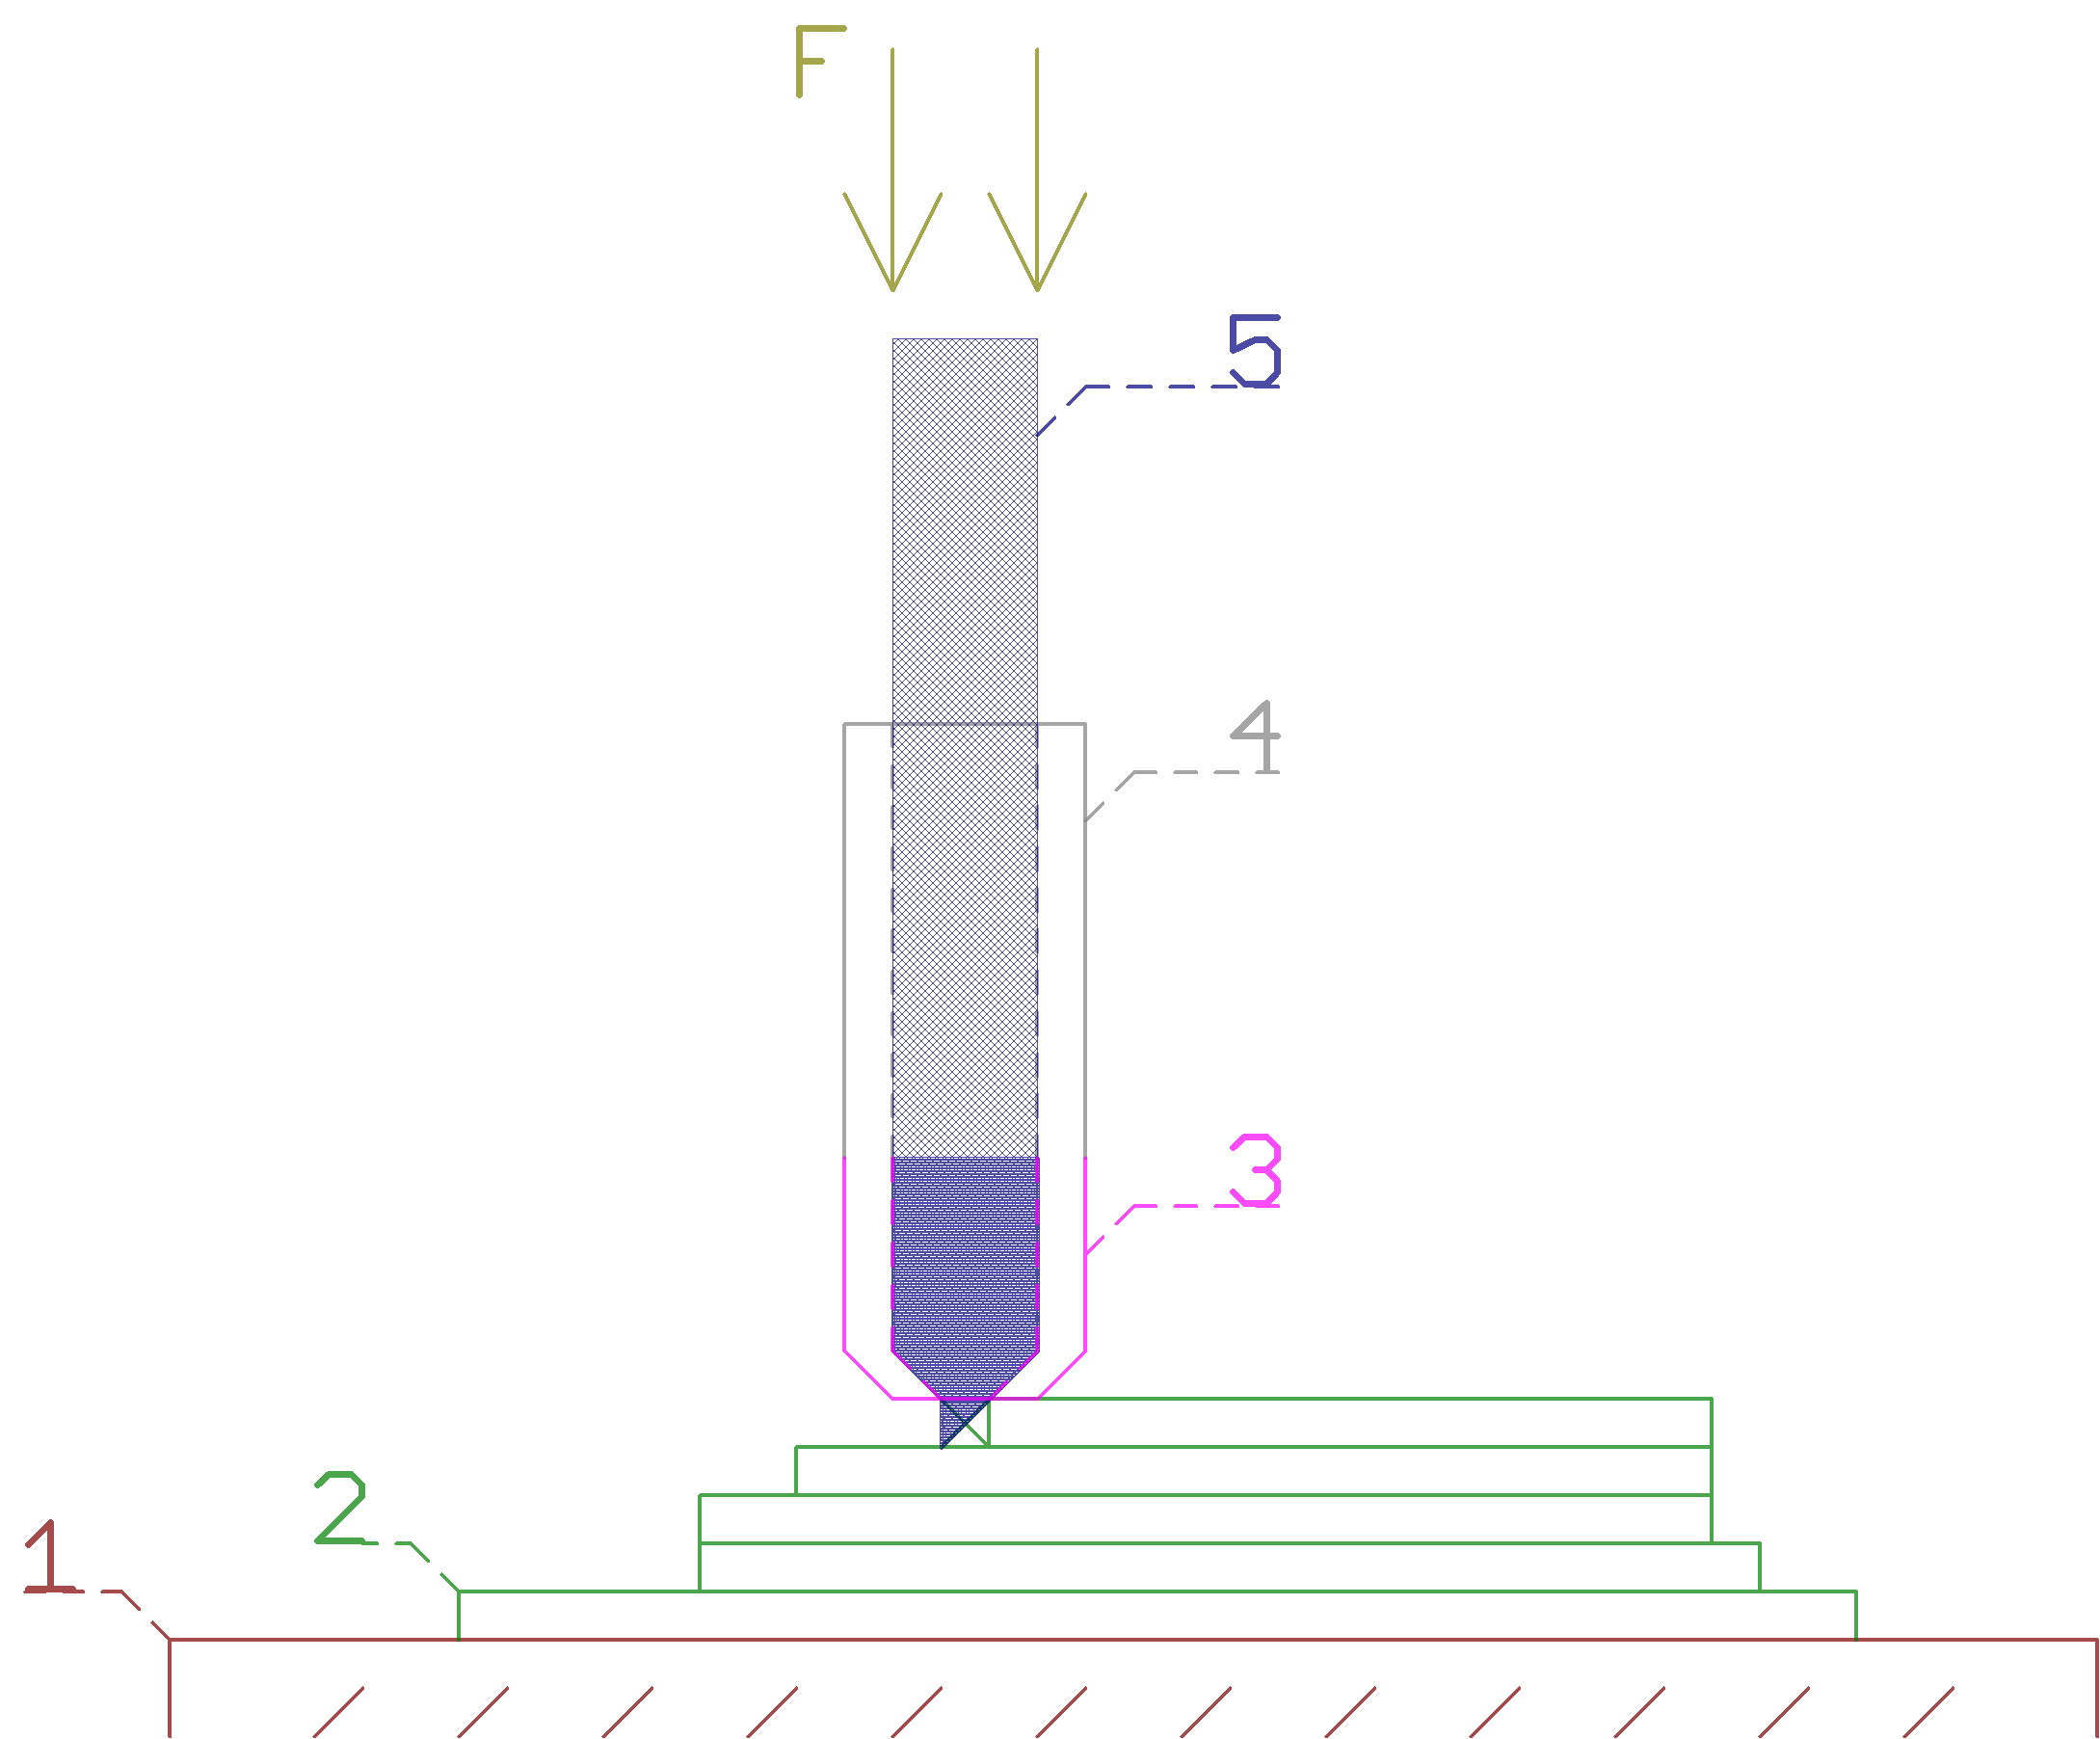
\includegraphics[width=9.5cm]{pics/fdm}
\caption{Princip technologie FDM. 1 - Tisková podložka, 2 - Již hotové vrstvy výsledného objektu, 3 - Horká zóna trysky, 4 - Tryska, 5 - Filament, F - Vtlačovací síla}
\end{center}
\end{figure}

\subsection{Vlastnosti technologie}
3D tisk, podobně jako jiné technologie má specifické vlastnosti, které ovlivňují charakter výsledného produktu. Ovlivněných vlastnostností je velmi mnoho, pro naši aplikaci se zaměříme na dielektrické (chceme vědět jaké bude mít výsledný produkt dielektrické vlastnosti, abychom ho byly schopni popsat, navrhovat a simulovat) a mechanické (produkt musí být možno pevně a stabilě ukotvit na pozici, a musí do něj být možno navázat elektromagnetickou vlnu známým způsobem). Je však nutno brát v potaz, že má i celou řadu vlastností, kterých lze využít pro vytvoření složitých struktur, které by nebylo možné jinými technologiemi jednoduše realizovat, například vnitřní uzavřené struktury. Některé z nich jsou pro dostatečně přesné aproximace dosažitelné v reálném časovém horizontu zcela náhodné, některé přímo ovlivňují námi velmi žádané parametry a můžeme je takto řídit.
\subsubsection{Vrstvy}
Pokud budeme uvažovat ideální podmínky (absolutně čisté prostředí bez kontaminace nechtěnými látkami, ideální filament, rovnoměrnou kontrolovanou distribuci tepla, atd...) stále je objekt tvořem z vrstev. Jelikož vždy vrtva, na které se aktuálně nanáší, je dokonce pod teplotou skelného přechodu, pro odstranění deformace vlivem sil jako gravitace, či tepelné roztažnosti, nedojde k dokonalému spojení polymerních řetězců mezi vrtvami. Při laminaci vrstev může také dojít ke kontaminaci produktu, jako například prachovými částicemi či vzduchovými kapsami. Toto se však dá zanedbat jelikož lze snadno stabilizovat okolní prostředí a minimalizovat vliv. 
Hlavní ovlivněné vlastnosti, pro naši aplikaci podstatné, jsou mechanické. Vždy je v ose vrstev rozložení mezne plasticity neuniformní, dochází tedy k plastické deformaci významně v těchto oblastech, což někdy může být problém z důvodu nutnosti splnění možnosti upevnění a realizovatelnosti produktu.
Z dielektrického hlediska tedy nebude ani relativní permitivita uniformně rozložená v jedné ose, vznikne tedy periodická stuktura. Tento vliv by bylo možné omezit buďto zvýšením diskretizačního kroku, tedy omezením počtu rozhraní, což může v jistých případech ovlivňovat vlastnosti celé struktury vzhledem růstu kvantizačního šumu, nebo naopak snížením kroku kdy již bude úroveň šumu blízká nule, což se bohužel negativně projeví na době tisku, to však v některých případech není problém. Výzkum popisu tohoto chování je však předmětem dalším.

\subsubsection{Vnitřní struktury}
Vlivem principu vrstvení je možno vytvářet vnitřní struktury definovaných tvarů, dokonce i selektivně, a takto velmi silně ovlivňovat pro nás důležité parametry.
Mechanické vlastnosti tímto lze slektivně měnit, například zpevněním montážních ovorů v technologickém okolí, což v našem případě není první v pořadí.
Dielektrické vlastnosti jsou tímto však velmi ovlivněny. Technologií je totiž možno vytvářet prakticky jakékoliv struktury uvnitř produktu ve zvolených místech, tedy například vytisknout Luneburgovu či Maxwell fish-eye čočku. Je však ale nutno provést výzkum na toto téma dostatečné podrobrý výzkum, jedná se totiž o skokové změny vlastností. Tyto změny poté vytváří rozhraní, kde dochází odrazům, které zatím modelovat a popsat je velmi komplexní úlohou.

\begin{figure}[h]
\begin{center}
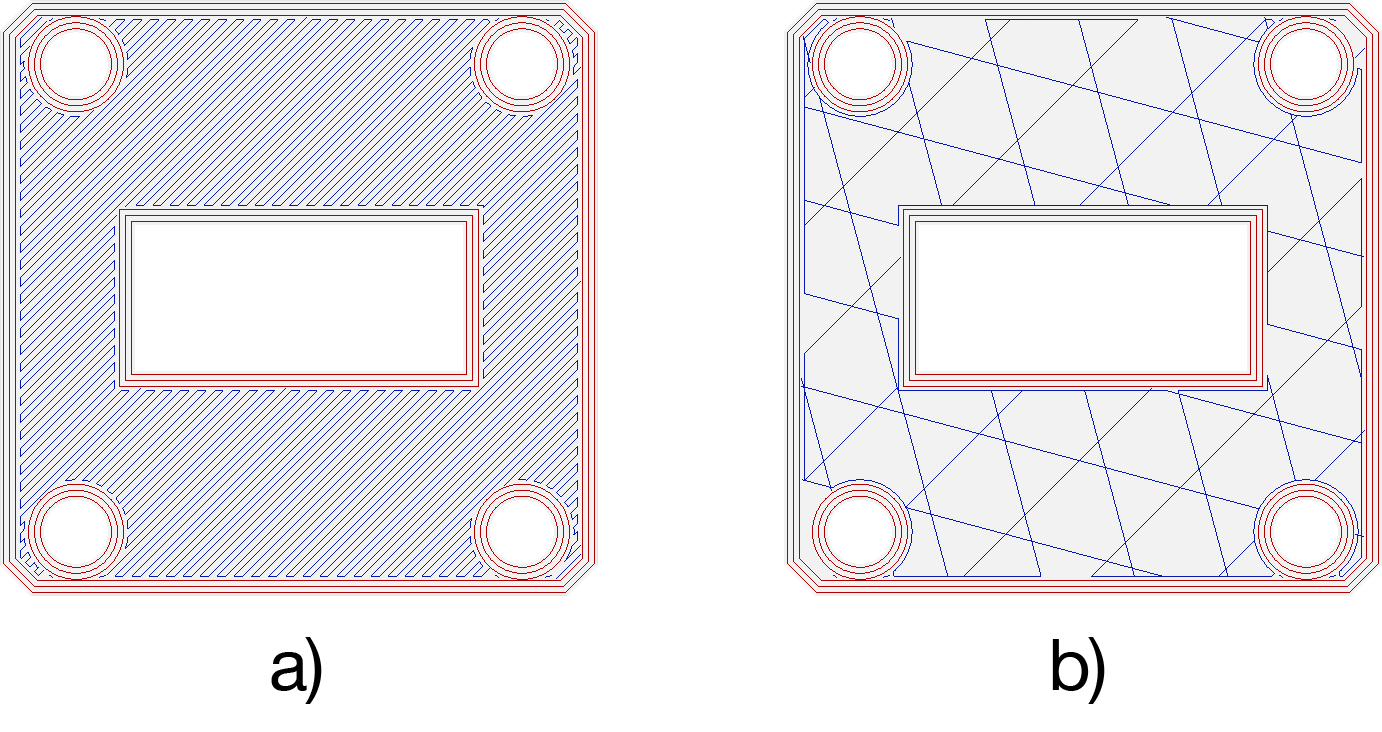
\includegraphics[width=9.5cm]{pics/fillcompare}
\caption{Porovnání různého motivu vrstvy, a) 100\,\% vyplň typem rectilinear, b) 20\,\% vyplnň typem cubic}
\end{center}
\end{figure}

\begin{figure}[h]
\begin{center}
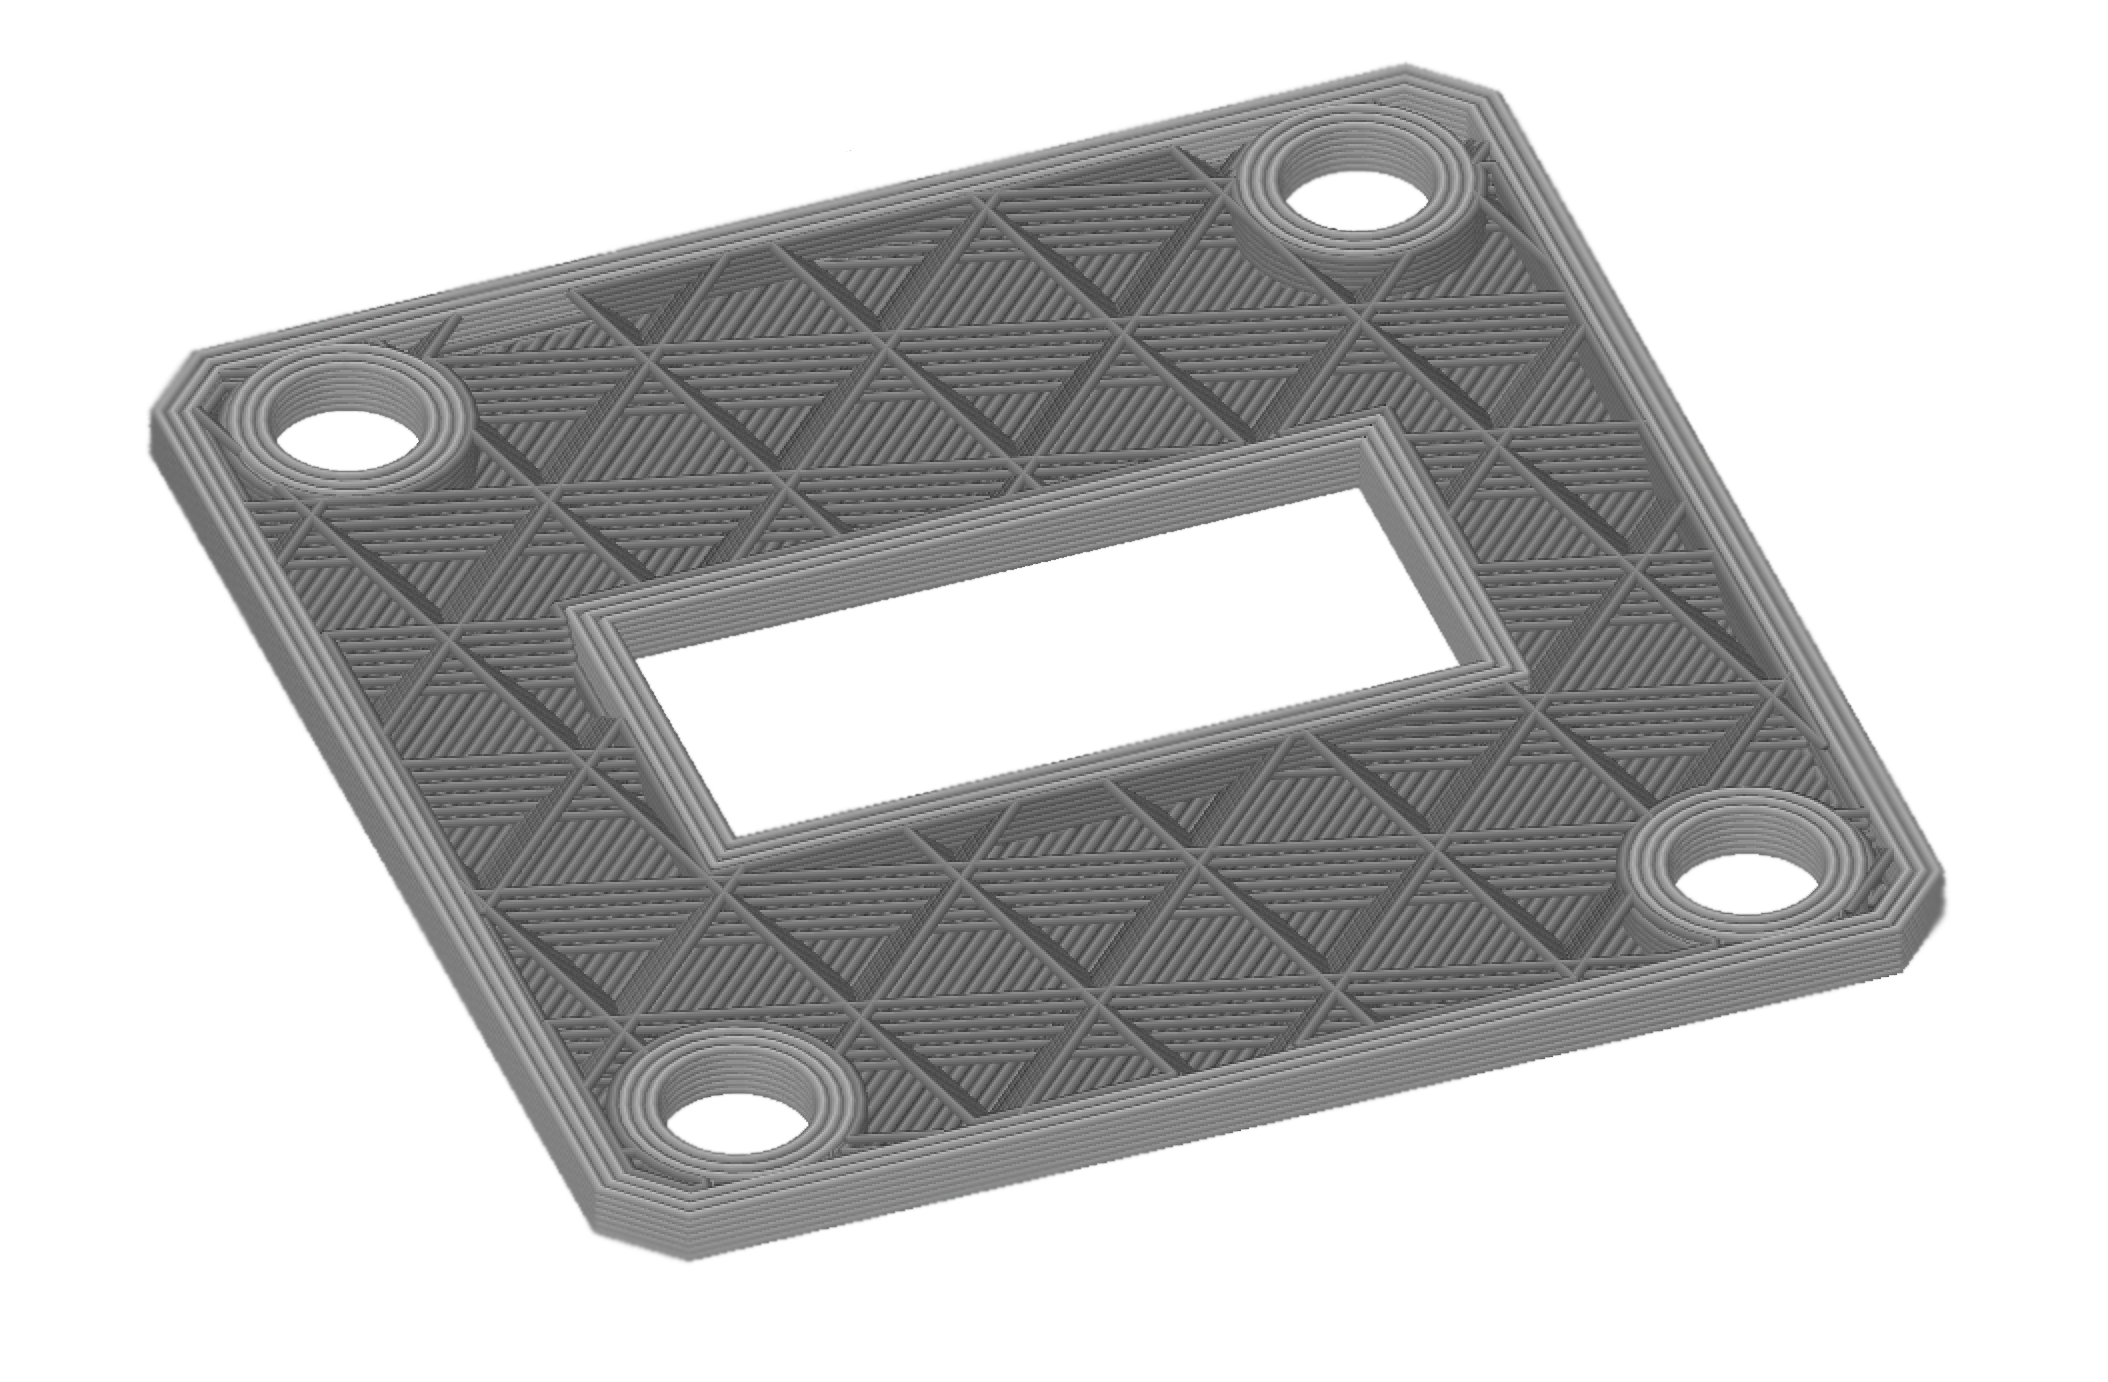
\includegraphics[width=9.5cm]{pics/6layer}
\caption{Náhled vrstev 1-6 struktury s kombinovanou výplní typu rectilinear (první dvě vrstvy) a cubic o rozdílné procentuální výplni}
\end{center}
\end{figure}

\subsection{Materiály využitelné pro vysokofrekvenční techniku}
Termopolymerních materiálů které by se daly využít je celá řada, teoreticky je možné uplatnit velké množství, prakticky však ale vyplývá otázka bezpečnosti, jelikož průchod některých polymerů procesem může uvolňovat nebezpečné látky, či v případě směsí její části.
Mezi nejrozšířenější patří PLA, ABS a PET, tyto materiály však lze uplatnit zejména v čočkách, či dielektrických rezonátorech, jelikož vykazují velmi malou vodivost. Objevují se ale stále nové směsy materiálů jako například PLA s výraznou příměsí grafénových šupin, či měděného prachu které v ideálním případě disponují velmi vysokou vodivostí.

\subsubsection{"Vodivé" materiály}



\section{Trychtýřová anténa}
Trychtýřová anténa patří mezi základní anténní struktury využívané jak samostatně, tak ve formě ozařovačů reflektorových antén, či v kombinaci s anténní čočkou. Těchto struktur existuje několik druhů, v našem případě se ale zaměříme na pyramidální trychtýřovou anténu.
Tento typ antény byl zvolen zejména kvůli své jednoduchosti a požadavkům na technologii výroby.

\subsection{Základní princip}
\subsection{Vlastnosti struktury}


\section{Anténní čočka}

\subsection{Základní princip}
\subsection{Vlastnosti struktury}




\section{Extrakce dielektrických parametrů}